\documentclass[a4paper]{usiinfbachelorproject}

\captionsetup{labelfont={bf}}
%%%%%%%%%%%%%%%%%%%%%%%%%%%% PACKAGES %%%%%%%%%%%%%%%%%%%%%%%%%%%%%
\usepackage{float}
\usepackage{amsmath}

%%% Main Body %%%

\author{Student's full name }

\title{\textbf{Project Title}}
\subtitle{Subtitle}
\versiondate{\today}

\begin{committee}
%With more than 1 advisor an error is raised...: only 1 advisor is allowed!
\advisor[Universit\`a della Svizzera Italiana, Switzerland]{ }{Firstname }{Lastname }
%You can comment out  these lines if you don't have any assistant
\coadvisor[Universit\`a della Svizzera Italiana, Switzerland]{ }{Firstname}{Lastname}

\end{committee}

\abstract { Abstract goes here ...
You may include up to six keywords or phrases. Keywords should be separated with semicolons. 
\\
\textbf{Keywords}:

}
\begin{document}
\maketitle
\tableofcontents\newpage
%\listoffigures\newpage

\section{\textbf{Introduction}}
Start writing your intro here. You can then use the following commands in your LaTeX document:
\cite{label} To insert a citation where label is the label of a bibliographic entry in a .bib file. For instance:\cite{Hamari}\\




\section{\textbf{Background}}
\subsection{\textbf{subsections}}
Explain all acronyms and abbreviations. For example, the first time an acronym is used, write it out in full and place the acronym in
parentheses. When using the Graphical User Interface (GUI) version, the use may...



\section{\textbf{Approach}}
\subsection{\textbf{The main idea}}
Some of the various techniques are listed below:

\begin{itemize}
	\item tech 1
	\item tech 2
\end{itemize}

\noindent You may write the formulas as follows:

\begin{equation}
	\phi(n) = (p-1) \cdot (q-1)\\
\end{equation}




To insert a figure use the following command:

\begin{figure}[h!]
	\center{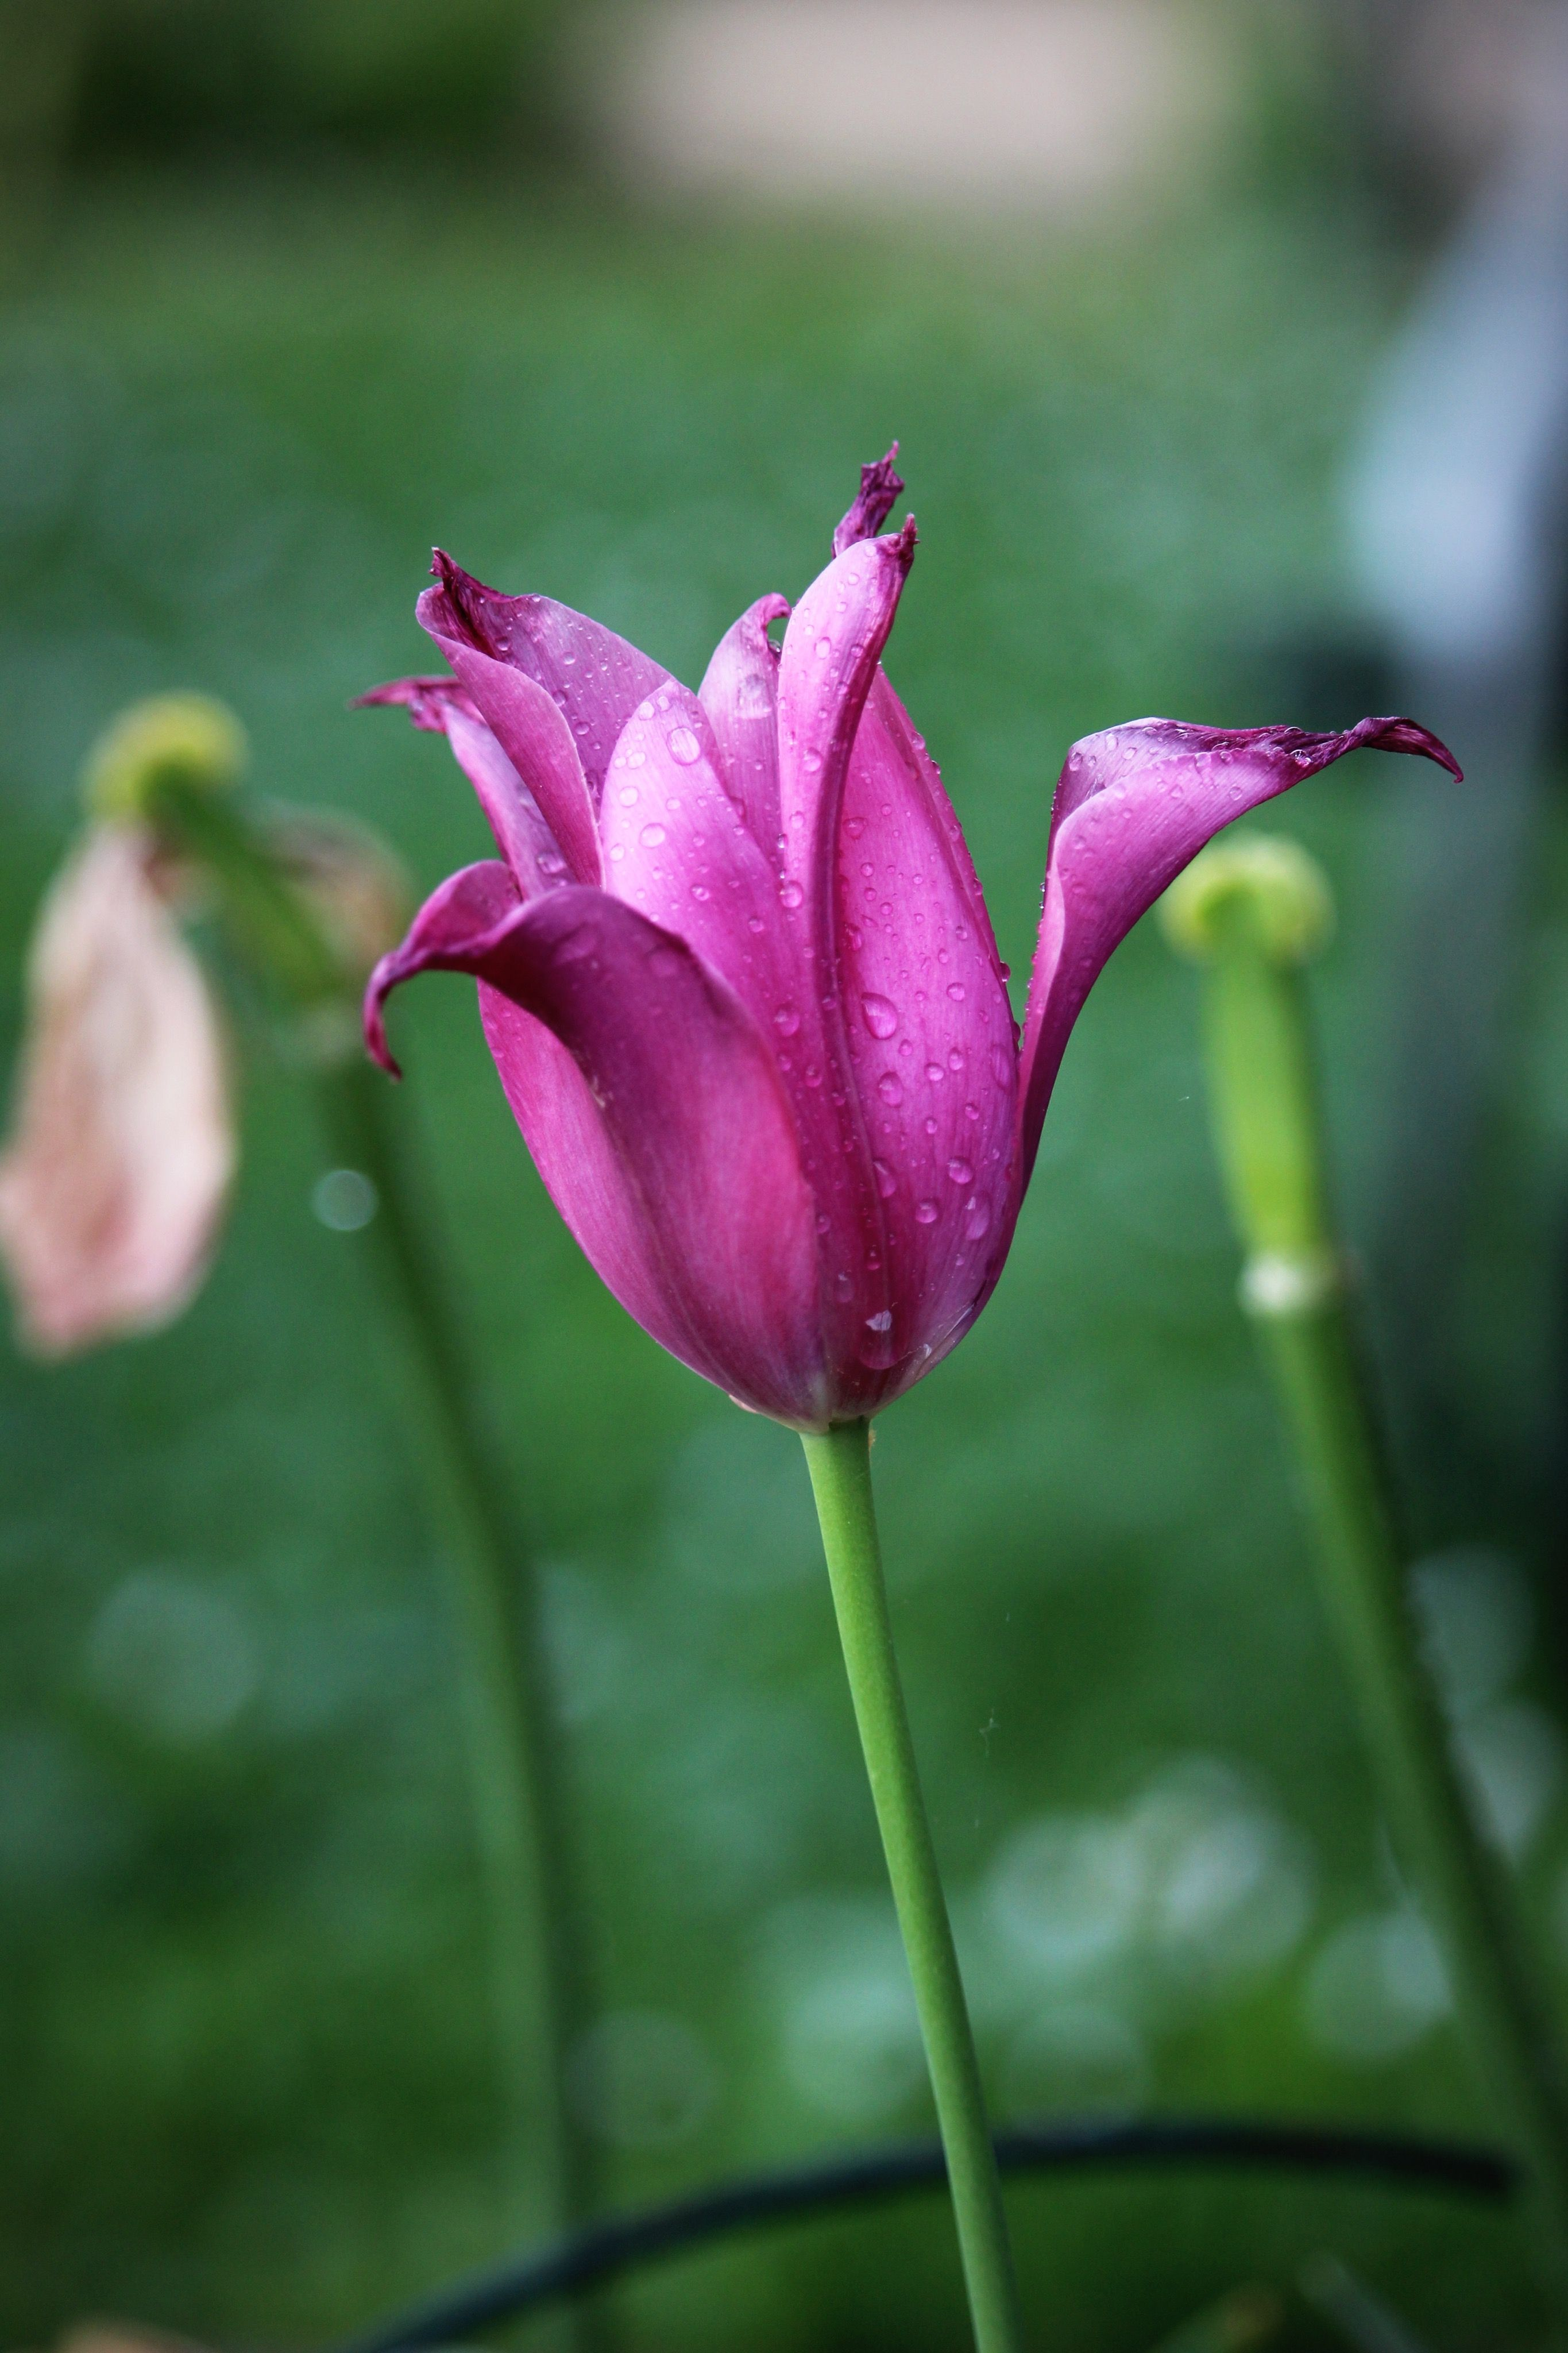
\includegraphics[scale=0.03 ]
		{figures/flower.jpg}}
	\caption{The caption of my figure}\label{fig:flower}
\end{figure}




\section{\textbf{Evaluation}}
\subsection{\textbf{Results}}
The experimental result goes here ... \footnote{https://www.usi.ch}. \\







\newpage
\section{\textbf{Future work}}

\section{\textbf{Summary}}
Future works goes here.






\newpage

%%%%% BIBLIOGRAPHY %%%%%
\bibliographystyle{abbrv}
\bibliography{references}

\end{document}
